\newcommand{\vect}[1]{\textbf{#1}}

\section{Introduction}

Рассматривается задача декодирования сигналов активности головного мозга и построения нейроинтерфейса, работающего с временными рядами как с непрерывными во времени. В качестве решения предлается использовать рекуррентные модели с модифицированным скрытым состоянием, которое определяется как решение обыкновенного дифференциального уравнения. Считается, что такой подход позволит повысить производительность обработки нерегулярных временных рядов, которые возникают при непостоянном контакте со считывающим устройством, а так же будет применим для передискретизации сигнала при низких частотах сэмплирования, поскольку доступные для широкого круга устройства обычно имеют невысокую частоту дискретизации. Кроме этого ожидается получение непрерывного представления сигнала для возможного дальнейшего использования в качестве признакового описания.  

Обычно нейроинтерфейс предполагает работу с данными многомерных временных рядов (сигналов активности головного мозга). Наиболее распространенными для регистрации сигналов являются неинвазивные методы на основе электроэнцефалографии, не требующие операции для установки датчиков, обладающие низкой стоимостью, высоким временными разрешением и простотой в настройке. 
\begin{figure}[!h]
	\centering
	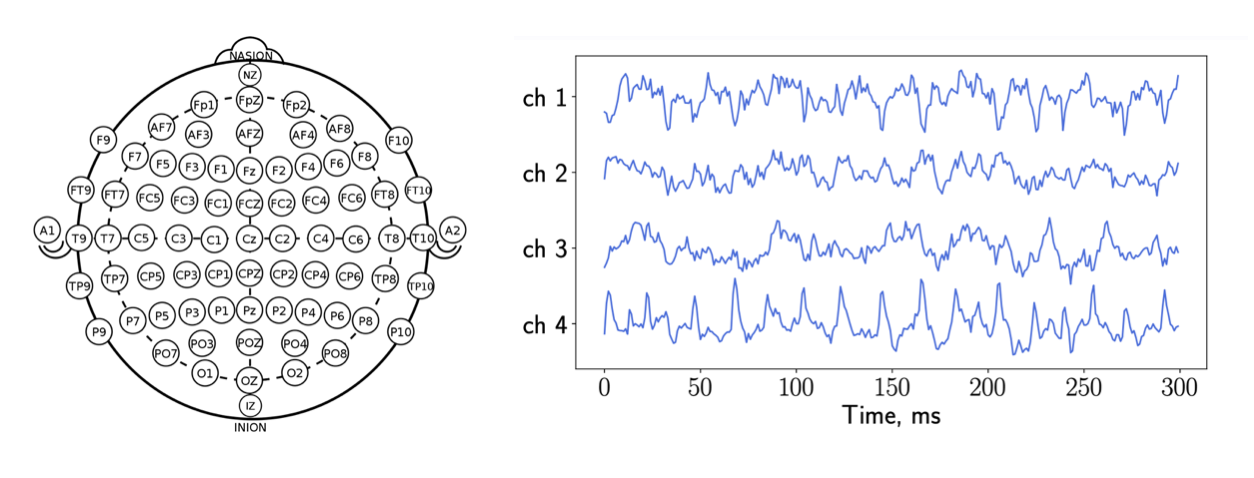
\includegraphics[width=0.8\textwidth]{chapters/varenik1/images/electodes-signal.png}
\end{figure}

При непрерывном представлении сигнала предполагается, что у нас есть некий процесс $V(t)$ - активность мозга и его реализация $\vect x_{t_i} \approx V(t_i)$ - наблюдаемый сигнал. Требуется построить функцию $f_{\vect X}(t): \mathbb{R}\to \mathbb{R}^E$, которая для любого момента времени сможет предоставить некоторое приближение сигнала или процесса $f_{\vect X}(t) \approx \vect x_t \approx V(t)$.

\textit{\textbf{Гипотеза.}}
Предлагается использовать скрытое состояние нейронных ОДУ (Neural ODE) в качестве непрерывныго представления сигнала.

\textit{\textbf{Критерии.}}
Скрытое состояние является непрерывным представлением сигнала, если оно удволетворяет следующим требованиям:
\begin{itemize}
    \item можно извлечь из модели и использовать самостоятельно как представление сигнала,
    \item сохраняет форму приближаемого процесса,
    \item позволяет получить значение в произвольный момент времени.
\end{itemize}
\section{References Review}
Статья~\cite{NEURIPS2018_69386f6b} является основной по теме Neural ODE. Вдохновившись синтаксической схожестью преобразования скрытого состояния в сети ResNet с формулой Эйлера для численного интегрирования ОДУ авторы предлагают механизм обратного распространения ошибки для обучения непрерывного в глубину аналога ResNet со скрытым состоянием, подчиняющимся ОДУ с параметризованной функцией динамики, параметры которой находятся минимизацией функции ошибки. В~\cite{NEURIPS2019_42a6845a} рассматривается ODE-модификация RNN для работы с нерегулярными по времени временными рядами. Идея состоит в доопределении скрытого состояния между наблюдениями решением нейронного ОДУ и корректировки полученной динамики в точках наблюдений по стандартному принципу RNN. Такое неявное добавление времени в состояние модели позволяет учесть информацию о временном интервале между наблюдениями, которая может быть полезна при обработке нерегулярных данных. Работа~\cite{DBLP:journals/corr/abs-2005-08926} посвящена еще одной модификации RNN для работы с данными, имеющими непостоянный шаг по временной шкале. В ней предлагается моделировать скрытое состояние управляемым дифференциальным уравнением, что позволяет получить непрерывную по отношению к входным наблюдениям функцию скрытого состояния. Для обработки длинных последовательностей нерегулярных временных рядов также имеются непрерывные по времени обобщения LSTM: в~\cite{DBLP:journals/corr/abs-2006-04418} рассматривается подход аналогичный ODE-RNN и показано, что предложенная архитектура аналогично стандартной не страдает от взрыва и затухания градиентов. В основе ~\cite{NEURIPS2019_952285b9} лежит построение ячейки памяти, представляющей непрерывное представление истории изменения сигнала в виде разложения на полиномы Лежандра, где в качестве коэффициентов используется компоненты состояния памяти LMU-LSTM.
\section{Main Part}

\subsection{Neural ODE}

Пусть задан процесс, который подчиняется некоторому неизвестному ОДУ и пусть известны несколько наблюдений вдоль траектории процесса, для простоты будем считать что их $2: t_0, t_1$ - в начале и в конце траектории:
\begin{equation}
    \frac{d\vect z}{dt} = f(\vect z(t), t), \{(\vect z_0, t_0), (\vect z_1, t_1)\} - \text{наблюдения}.
\end{equation}

Нужно найти аппроксимацию функции динамики $f(\vect z(t), t, \theta)$. 
В качестве аппроксиманта выступает нейронная сеть с параметрами $\theta$. Эволюция системы запускается из начального состояния на время $t_1 - t_0$ с какой-то параметризованной функцией динамики используя любой метод эволюции ОДУ. После того как система окажется в новом состоянии $\hat{\vect z}_1$ оно сравнивается с истинным  $\vect z_1$ и разница минимизируется поиском оптимальных параметров методом обратного распространения ошибки:
\begin{equation}
    L(\vect z(t_1)) = L(\vect z(t_0) + \int\limits_{t_0}^{t_1} f(\vect z(t), t, \theta))dt = L(ODESolver(\vect z(t_0), f, t_0, t_1, \theta)).
\end{equation}

Чтобы минимизировать $L$ нужно уметь эффективно проводить непрерывный по времени backpropagation. Для начала определим, как градиент функции потерь зависит от скрытого состояния:
\begin{equation}
    \vect a(t) = \frac{\partial L}{\partial \vect z(t)},
\end{equation}
эта величина называется сопряженным состоянием. Его динамика задается другим ОДУ:
\begin{equation}
    \frac{d\vect a(t)}{dt} = -\vect a(t)^T\frac{\partial f(\vect z(t), t, \theta)}{\partial \vect z},
\end{equation}
\begin{equation}
    \vect a(t_0) = \vect a(t_1) - \int\limits_{t_1}^{t_0} \vect a(t)^T\frac{\partial f(\vect z(t), t, \theta)}{\partial \vect z} \text{ при } \vect a(t_1) = \frac{dL}{d\vect z(t_1)}.
    \label{eq1}
\end{equation}

В общем случае нужно найти градиенты по всем входным параметрам решателя ОДУ. Рассмотрим как найти градиенты по $\vect z_0$ и $\theta$ за один проход. 

Для этого вводится аугментированное состояние - обычное состояние $\vect z$ к которому добавили $\theta$. Его динамика тривиальным образом определяется из оригинальной динамики:
\begin{equation}
    \frac{d}{dt}\begin{bmatrix}
        \vect z \\
        \theta \\
        \end{bmatrix}(t) = f_{aug}([\vect z, \theta]) := \begin{bmatrix}
        f([\vect z, \theta, t]) \\
        \vect 0 \\
    \end{bmatrix},
\end{equation}

сопряженное состояние к такому аугментированному:
\begin{equation}
    \vect a_{aug} := \begin{bmatrix}
    \vect a \\
    \vect a_{\theta} \\
    \end{bmatrix},
    \vect a_{\theta} := \frac{dL}{d\theta(t)}.
\end{equation}

Посчитав градиент аугментированной динамики:
\begin{equation}
    \frac{\partial f_{aug}}{\partial [\vect z, \theta]} =  \begin{bmatrix}
    \frac{\partial f}{\partial \vect z}&\frac{\partial f}{\partial \theta}\\
    \vect 0&\vect 0\\
    \end{bmatrix}(t),
\end{equation}
получим дифференциальное уравнение для аугментированного сопряженного состояния:
\begin{equation}
    \frac{d\vect a_{aug}(t)}{dt} = \begin{bmatrix}
    \vect a(t) & \vect a_{\theta}(t)
    \end{bmatrix} \frac{\partial f_{aug}}{\partial [\vect z, \theta]}(t) = - \begin{bmatrix}
    \vect a(t)\frac{\partial f}{\partial \vect z} & \vect a(t)\frac{\partial f}{\partial \theta}
    \end{bmatrix}.
\end{equation}

Исходя из полученной динамики мы легко можем определить градиент по $\theta$ как решение ДУ назад во времени для $\theta$-компоненты:
\begin{equation}
    \frac{dL}{d\theta} = \vect a_{\theta}(t_0) =  - \int\limits_{t_1}^{t_0}\vect a(t)^T\frac{\partial f(\vect z(t), t, \theta)}{\partial \theta}dt \text{ при } \vect a_{\theta}(t_1) = \vect 0.
    \label{eq2}
\end{equation}

Градиент по $t$ можно найди аналогичным образом добавив его в аугментированное состояние. Таким образом, чтобы получить требуемые градиенты нужно вычислить \ref{eq1} и \ref{eq2} назад во времени начиная с $t_1$.

Все необходимые градиенты можно получить за один проход алгоритма непрерывного обратного распространения с использованием решения аугментированного ДУ:

\begin{figure}[!h]
	\centering
	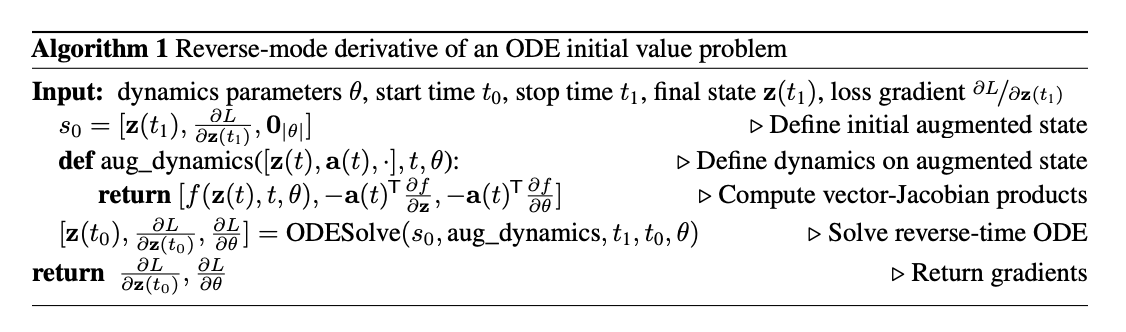
\includegraphics[width=0.9\textwidth]{chapters/varenik1/images/backpropagation-algo.png}
\end{figure}

Ввиду того, что вычисление рассмотренных двух интегралов требует знания $\vect z(t)$ на всей траектории и с учетом того, что решатель ОДУ может выводить значения состояния для некоторого набора отсчетов времени предлагается запускать эволюцию состояния $\vect z(t)$ вместе с сопряженным состоянием назад во времени. Тогда распространение назад сопряженного состояния разбивается на части и проводится корректировка в точках наблюдений в направлении соответствующих градиентов (см. рис. \ref{fig:im1}).

\begin{figure}[!h]
	\centering
	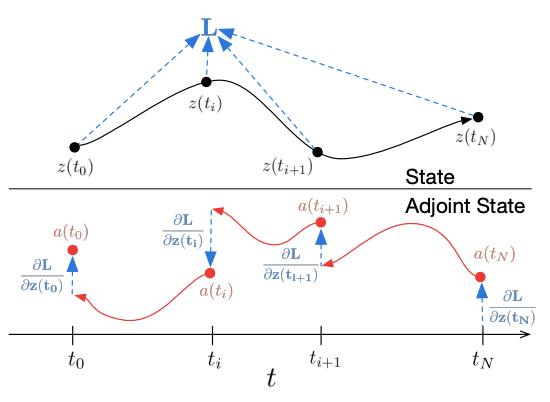
\includegraphics[width=0.45\textwidth]{chapters/varenik1/images/backpropagation.png}
	\caption{Непрерывное распространение назад.}
	\label{fig:im1}
\end{figure}

\newpage
\subsection{ODE-RNN}

Рассмотрим нерегулярный временной ряд:
\begin{equation*}
    \vect X = \{(\vect x_i, t_i)\}_{i=0}^N, t_i\in \mathbb{R}, t_0 \le \dots \le t_N, \Delta_t = t_{i+1} - t_{i} \neq const, \vect x_i \in \mathbb{R}^E
\end{equation*}

\begin{wrapfigure}{r}[8pt]{.45\textwidth}
    \centering
    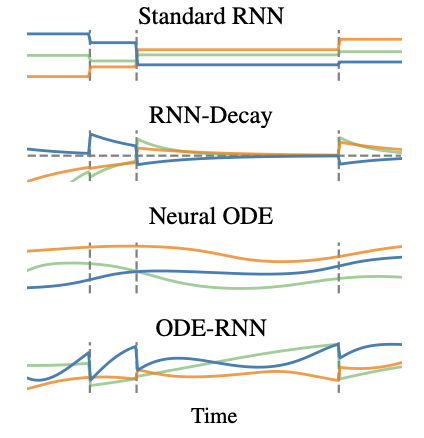
\includegraphics[scale=0.9]{chapters/varenik1/images/ode-rnn.png}
    \caption{Динамика скрытых состояний разных размерностей. Вертикальные линии соответствуют временам наблюдений.}
\end{wrapfigure}

Самым распространенным подходом для анализа регулярных последовательностей являются рекуррентные модели. Но они в своем построении предполагают равномерный одинаковый шаг между наблюдениями, и таким образом не способны извлекать информацию о времени измерения, которая может быть полезна в качестве описания при анализе нерегулярных данных. Следовательно, нужно определить зависимость состояния от расстояния во времени между наблюдениями. Естественным в таком случае кажется введение модели с непрерывным скрытым состоянием. 

Один из простых вариантов учета дельты - добавить ее в качестве входной переменной в ячейку RNN, но тогда остается открытым вопрос как определить состояние между моментами наблюдений:
\begin{equation*}
    \vect h_i = RNNCell(\vect h_{i-1}, \Delta_t, \vect x_i), \text{ }\Delta_t = t_i - t_{i-1};
\end{equation*}

Следующее решение - определить динамику между наблюдениями через экспоненциальный спад:
\begin{equation*}
    \vect h_i = RNNCell(\vect h_{i-1} \exp(-\tau \Delta_t), \vect x_i), \text{ } \tau - \text{параметр спада};
\end{equation*}

Однако, экспериментально было показано, что такая модификация не дает улучшения в производительности по сравнению со стандартной архитектурой. Поэтому, предлагается вводить непрерывную во времени динамику через решение  Neural ODE: 
\begin{equation*}
    \vect h_0, \dots, \vect h_N = ODESolver(f_{\theta}, \vect h_0, (t_0, \dots, t_N));
\end{equation*}

Обычный подход ODE хоть и задает сложную траекторию скрытого состояния, но она определяется лишь начальным состоянием и не адаптируется к поступающим наблюдениям. Следовательно, предлагается модификация преобразования состояния в рекуррентной сети, в которой состояние между наблюдениями определяется как решение ODE, а в точках наблюдений происходит обновление, аналогичное стандартной RNN:
\begin{align*}
   & \vect h_i' = ODESolver(f_{\theta}, \vect h_{i-1}, (t_{i-1}, t_i)),\\
   & \vect h_i = RNNCell(\vect h_i', \vect x_i).
\end{align*}

\subsection{Neural CDE}

Рассмотрим другое расширение обычных нейронных уравнений, способное предоставить непрерывное представление сигнала, учитывающее входящие наблюдения, которые могут быть как нерегулярными, так и частично наблюдаемыми - нейронные управляемые уравнения.

Пусть $S:[t_0, t_N] \to \mathbb{R}^{E+1}$ - натуральный кубический сплайн с узлами в $t_0, \dots, t_N$, $S_{t_i} = (\vect x_i, t_i)$, который по построению является аппроксимацией процесса с реализациями, представленными в $\vect X$. 

Пусть $f_{\theta}: \mathbb{R}^d \to \mathbb{R}^{d\times (E+1)}$, $g_{\theta}: \mathbb{R}^{E+1} \to \mathbb{R}^{d}$ - нейронные сети, зависящие от параметра $\theta$, $d$ - размерность скрытого пространства.

Тогда скрытое состояние определяется, как решение управляемого ДУ:
\begin{equation}
   \vect z_t = \vect z_{t_o} + \int\limits_{t_0}^t f_{\theta}(\vect z_{\tau})dS_{\tau}, t\in (t_0, t_N], \text{ где } \vect z_{t_0} = g_{\theta}(\vect x_0, t_0).
\end{equation}

\begin{figure}[!h]
	\centering
	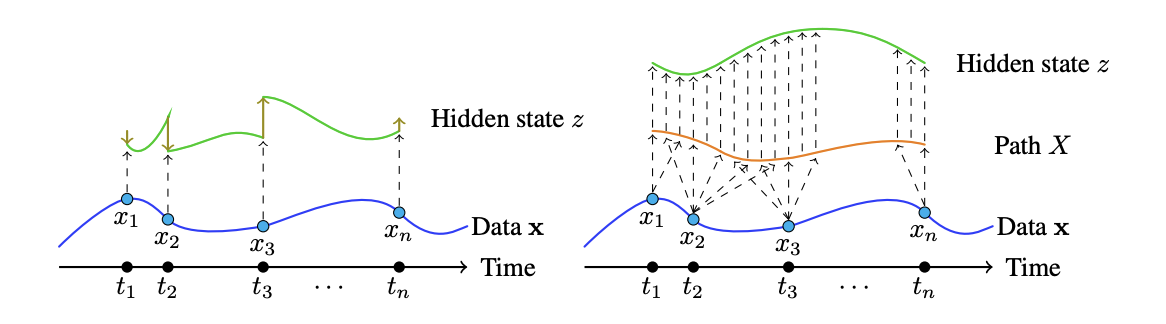
\includegraphics[width=0.8\textwidth]{chapters/varenik1/images/neural-cde.png}
	\caption{Сравнение скрытого состояния ODE-RNN и Neural CDE.}
	\label{fig:im2}
\end{figure}

По своей архитектуре рассмотренный подход также является рекуррентной моделью, но главное отличие от предыдущей архитектуры состоит в непрерывности скрытого состояния по отношению к наблюдениям см. рис. \ref{fig:im2}).

\subsection{ODE-LSTM}

Ввиду известной проблемы взрыва и затухания градиентов для RNN, их применение становится невозможным для обработки длинных последовательностей. Общепринятым решением является модель LSTM. 

Скрытое состояние - пара $(\vect c_t, \vect h_t)$, $\vect c_t$ - состояние долгосрочной памяти, $\vect h_t$ - обычное скрытое состояние.

Функция обновления $f_{\theta}(\vect x_{t+1}, (\vect c_t, \vect h_t)) \mapsto (\vect c_{t+1}, \vect h_{t+1})$ определяется набором уравнений:
\begin{align*}
    & \vect z_{t+1} = tanh(\vect W_z \vect x_{t+1} + \vect R_z\vect h_t+\vect b_z),\\
    & \vect i_{t+1} = \sigma(\vect W_i\vect x_{t+1} + \vect R_i \vect h_t + \vect b_i),\\
    & \vect f_{t+1} = \sigma(\vect W_f\vect x_{t+1} + \vect R_f \vect h_t + \vect b_f + \vect 1),\\
    & \vect o_{t+1} = \sigma(\vect W_o\vect x_{t+1} + \vect R_o \vect h_t + \vect b_o),\\
    & \vect c_{t+1} = \vect z_{t+1}\odot \vect i_{t+1} + \vect c_t\odot \vect f_{t+1},\\
    & \vect h_{t+1} = tanh(\vect c_{t+1})\odot \vect o_{t+1}.
\end{align*}

Аналогично RNN производится ODE модификация LSTM, предоставляющая непрерывный учет времени в скрытом состоянии:
\begin{align*}
    & (\vect c_{t+1}, \vect h_{t+1}') = LSTM(\theta_l, (\vect c_t, \vect h_t), \vect x_{t+1})),\\
    & \vect h_{t+1} = ODESolver(f_{\theta}, \vect h_{t+1}', t_{t+1} - t_{t}),\\
    & \vect o_{t+1} = \vect h_{t+1}\vect W_{output} + b_{output}.
\end{align*}

\subsection{LMU-LSTM}

Рассмотрим еще одну модификацию LSTM - Legendre Memory Units. Главным компонентом является ячейка памяти, описываемая системой d связанных ОДУ:
\begin{equation*}
    \theta \dot{\vect c(t)} = \vect A\vect c(t) + \vect bu(t),
\end{equation*}
где $\vect c(t)\in \mathbb{R}^d$ - состояние долгосрочной памяти,
$u_t \in \mathbb{R}$ - история изменения входящего сигнала.

Наилучшие матрицы $(\vect A, \vect b)$ получаются с помощью аппроксимантов Паде:

\begin{center}
    $\vect A = [a]_{ij} \in \mathbb{R}^{d\times d}, \text{ } a_{ij} = (2i+1)
    \begin{cases}
        -1 & i < j \\
        (-1)^{i-j+1} & i\ge j\\
    \end{cases}$,
\end{center}
\begin{center}
    $\vect b = [b]_i \in \mathbb{R}^{d\times 1},  \text{ } b_i = (2i+1)(-1)^i,  \text{ } i, j \in [0, d-1]$.
\end{center}

Основное свойство данной динамической системы заключается в том, что $\vect c(t)$ представляет скользящее окно $u$ по полиномам Лежандра степени до $d-1$:

\begin{equation*}
    u(t-\theta') \approx \sum\limits_{i=0}^{d-1} \mathcal{P}_i\Bigg(\frac{\theta'}{\theta}\Bigg)c_i(t), \text{ } 0\le \theta' \le \theta, \text{ } \mathcal{P}_i(r) = (-1)^i\sum\limits_{j=0}^i\binom{i}{j}\binom{i+j}{j}(-r)^j
\end{equation*}

где $\mathcal{P}_i(r)$ - сдвинутые полиномы Лежандра.
\begin{figure}[!h]
	\centering
	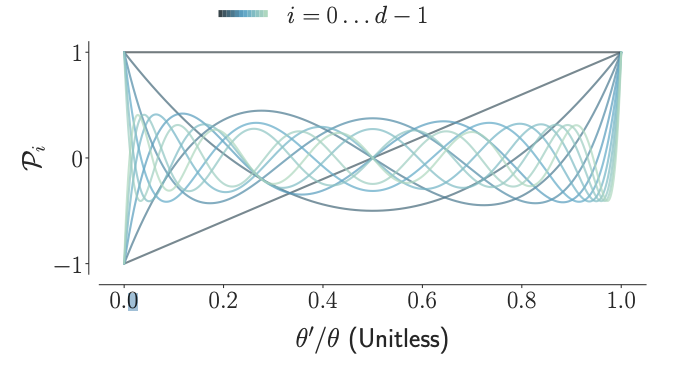
\includegraphics[width=0.55\textwidth]{chapters/varenik1/images/legendre.png}
\end{figure}

\subsection{Применение к декодированию}

Здесь приведены результаты работы\footnote{\url{http://www.machinelearning.ru/wiki/images/6/62/Samokhina2021MSThesis.pdf}} по построению непрерывного представления. Построение осуществлялось в рамках решения задачи классификации потенциалов $P300$, где непрерывное представление извлекалось из скрытого состояния алгоритмов классификации. $P300$ это потенциал активности мозга, в котором пик соответствует реакции на внешний стимул. 

Было показано, что скрытое состояние Neural CDE отвечает всем поставленным критериям непрерывного представления сигнала. Состояние $z(t)$ не является точным описанием процесса $V(t)$, но сохраняет его форму.
	
\begin{figure}[ht]%
    \centering
    \subfloat[Потенциал P300.]{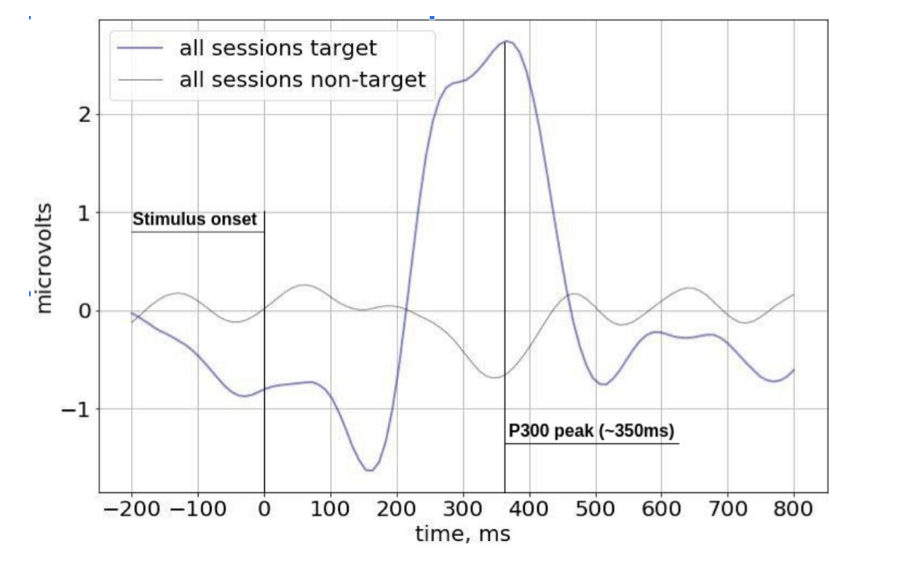
\includegraphics[width=0.47\linewidth]{chapters/varenik1/images/p300.png}}\qquad
    \subfloat[Непрерывное представление сигнала.]{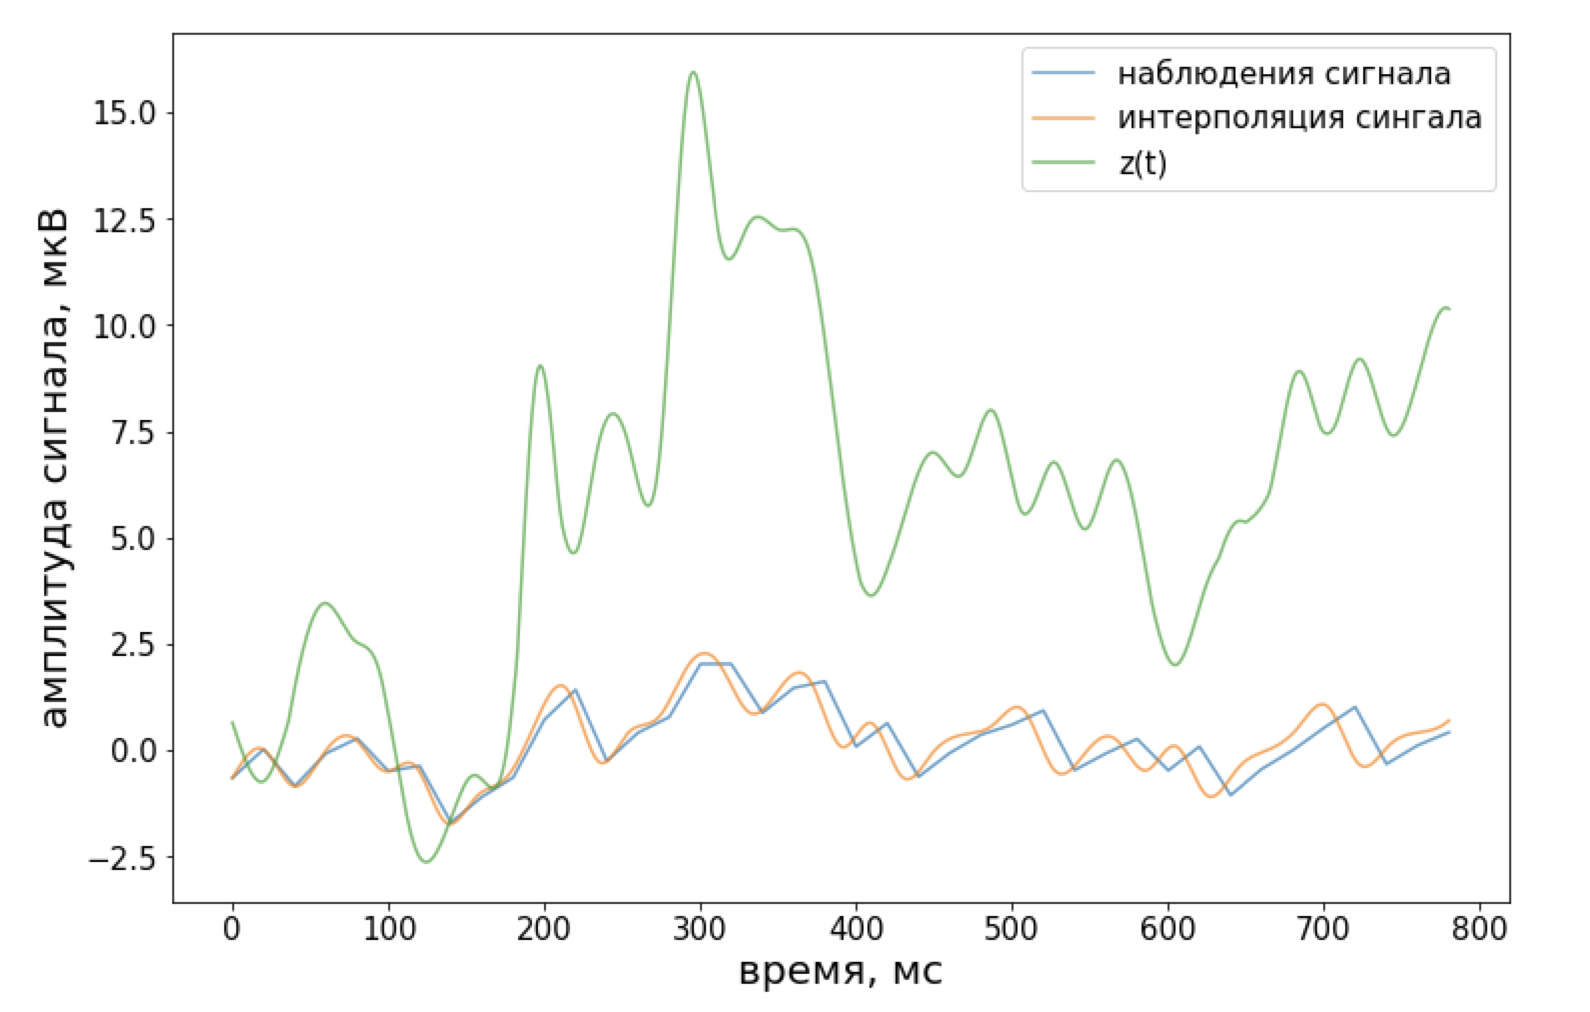
\includegraphics[width=0.46\linewidth]{chapters/varenik1/images/result.png}}
\end{figure}

\section{Questions To Discussion}
\begin{enumerate}
    \item Для чего нужно непрерывное по времени представление сигнала.
    \item Как работает непрерывный метод обратного распространения ошибки.
    \item Почему стандартная RNN не подходит для анализа нерегулярных временных рядов.
    \item В чем преимущество Neural CDE над ODE-RNN.
\end{enumerate}